%----------------------------------------------------------------------------
\chapter{Gravitációs hatásából származó terhelés kompenzációja}
\label{sec:grav_komp}
%----------------------------------------------------------------------------

A bevezetőben, illetve a szakdolgozatban elkészített telemanipulátor esetében is megfogalmaztam, hogy figyelembe vettem annak lehetőségét, hogy a gravitációs hatásából származó terhelésre kompenzációs lehetőséget tervezzek. A tervezéshez korábban, egy adott típusú megoldást vettem figyelembe, azonban ebben a fejezetben nagyon röviden a leggyakrabban előforduló lehetőségeket is bemutatom. A fejezetet azzal zárom, hogy a megépített telemanipulátornál melyik megoldást alkalmaztam.

\section{Kompenzációs lehetőségek}
%----------------------------------------------------------------------------

Az elvégzett kutatásaim alapján a kompenzációs lehetőségeket két nagy csoportba sorolják, vannak az aktív illetve a passzív elemeket felhasználó lehetőségek.\cite{gravkomp}

\begin{figure}[!h]
\centering
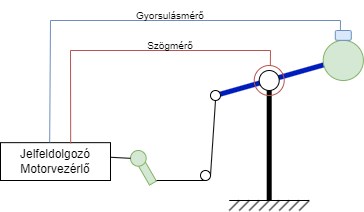
\includegraphics[width=75mm, keepaspectratio]{figures/Diagrammok/Kompenzacios_lehetosegek_aktiv}
\caption{Aktív kompenzációs lehetőségek szemléltetése}
\label{fig:Kompenzacios_lehetosegek_aktív}
\end{figure}

Az aktív rendszerek valamilyen szenzorral gyűjtött jel alapján aktuátorokkal valósítják meg a kompenzációt. A rendszer felépítésében összetett, ugyanis szenzorból, jelfeldolgozó rendszerből, teljesítmény elektronikából és valamilyen beavatkozó szervből kell felépíteni. Analógia alapján tekinthetjük úgy, hogy egy kis robotot kell felépíteni. Ennek a kis robotnak pedig az a feladata - az én esetemben -, hogy a telemanipulátor karjain a gravitációs erő ne érződjön.\cite{gravkomp}


A passzív rendszerek pedig a fizika alaptörvényeit használják fel. Három kompenzációs erőt létrehozó elemből állhatnak, ezek pedig tömeg, rugó, vagy csillapító elem. Ezeknek a végtelen kombinációjával lehet találkozni a mérnöki életben. A következő ábrán bemutatom a legegyszerűbb és legelterjedtebb megoldásokat, amik alapján én is tovább haladtam.\cite{gravkomp}

\begin{figure}[!ht]
\centering
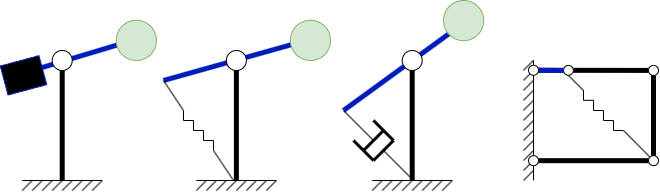
\includegraphics[width=125mm, keepaspectratio]{figures/Diagrammok/Kompenzacios_lehetosegek_passziv}
\caption{Passzív kompenzációs lehetőségek szemléltetése}
\label{fig:Kompenzacios_lehetosegek_passziv}
\end{figure}

Az első a tipikus ellensúlyos rendszer, amikor a csuklópont körül kiegyensúlyozzuk a kar két oldalát. Ennek eredményeképpen bármelyik állapotban megállítjuk a rendszert egyensúlyban marad. A második egy rugós megoldás, ez a típusú kompenzáció a test stabil állapotának pozícióját változtatja meg. A stabil pont az lesz, ahol a rugóerő és a nehézségi erő egyensúlyba kerül. A harmadik megoldás egy csillapítóval egy ellenállást tesz a rendszerbe. Rezgéstanból megtanulva a csillapítási erő nagyobb, mint a nehézségi erő akkor a rendszer nyugalomban van, ha kisebb akkor a rendszer a különbség arányában a stabil pont irányába mozog. A negyedik megoldás egy szemléltetés. Ebben az esetben összetettebb rendszer kinematikai kialakítását lehetséges úgy megadni, hogy a kinematikai elemek egymáshoz viszonyítottan tudják a kompenzációt létrehozni.\cite{gravkomp}

Fontos azonban megjegyezni, hogy a fent bemutatott megoldások lehetnek tömegkompenzációs lehetőségek. A nehézségi erőből fakadó terhelés kompenzációja megoldható ezekkel, de ez sokkal összetettebb mechanikai ismeretet is igényelhet. A következő példán szemléltetem, hogy mi a tömeg kompenzáció és mi a nehézségi erő kompenzációja.\cite{vezetekellen}

\begin{figure}[!ht]
\centering
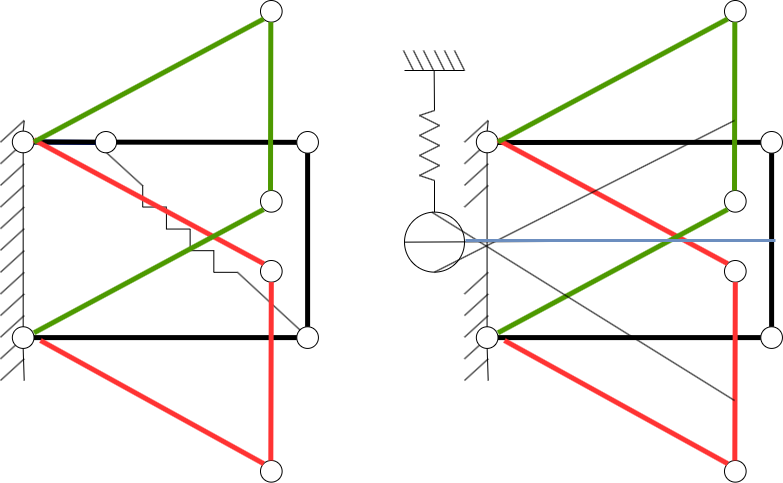
\includegraphics[width=125mm, keepaspectratio]{figures/Diagrammok/Tomeg_VS_Gravkomp}
\caption{Tömegkompenzációs és a nehézségi erő kompenzációjának szemléltetése}
\label{fig:Tomeg_VS_Gravkomp}
\end{figure}

A baloldali esetben a középső állásban van nyugalmi helyzetben a kinematikai rendszer, a zöld  és a piros kitérítés esetében is vissza fog állni a stabil helyzetbe. Itt a rugó megnyúlását használjuk fel. A jobboldali esetben viszont egy olyan bonyolultabb mechanikai rendszer dolgozik, ahol a középső állapotban van a kék karnak a legnagyobb kompenzációs hatása a két szélső helyzetben a baloldalon található kényszerpályás idomnak köszönhetően ugyanolyan mértékben csökken a kompenzációs hatás. A második példában fontos kiemelni, hogy mindkét irányba csökken ez a hatás, míg az első példában az egyik irányba nő a másikba csökken.

\section{Telemanipulátoron alkalmazható kompenzáció}
%----------------------------------------------------------------------------

Az előzőekben bemutatott kutatási eredményeim alapján egyértelmű volt számomra milyen típusú kompenzációs megoldásokat kell figyelembe vennem a tervezés során.

A következő ábrán látható is milyen elrendezésben lenne a legegyszerűbb megvalósítani azt, hogy a telemanipulátort minél könnyebben lehessen használni. Az első feltételként azt támasztottam, hogy két parallelogramma kinematikai elrendezést építenék be. A későbbiekben számos előnyére kitérek, de jelen esetben a rugós és a ellensúlyos rendszer komplexen megvalósíthatóak lennének és nem kell minden egyes karon külön tervezni ezt a lehetőséget, hanem egységes lenne. A másik nagy előnye, hogy lehetőséget ad a prototípus gyártásra, azaz kipróbálhatok többféle megoldást a későbbiekben.\cite{gravkomp}

\begin{figure}[!ht]
\centering
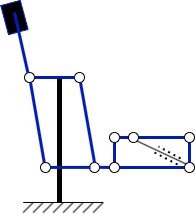
\includegraphics[width=55mm, keepaspectratio]{figures/Diagrammok/Megvalositott_kompenzacio}
\caption{Megvalósított kompenzációs rendszer}
\label{fig:Megvalositott_kompenzacio}
\end{figure}

%TODO ellensúly mérete

A diploma dolgozatom leadásának pillanatában az első paralelogrammás kinematikai rendszert ellensúlyos megoldással szereltem fel. A második paralelogrammás kinematikai rendszerbe egy rugós mechanikát helyeztem, ezzel a középső állapotba toltam a rendszer stabil pontját.Ide a bonyolult kinematikai rendszert ami lehetővé tenné a gravitációs hatásból származó nehézségi erő kompenzációját nem volt időm elkészíteni, de mindenképpen szeretném megvalósítani a későbbiekben.

\begin{figure}[!ht]
\centering
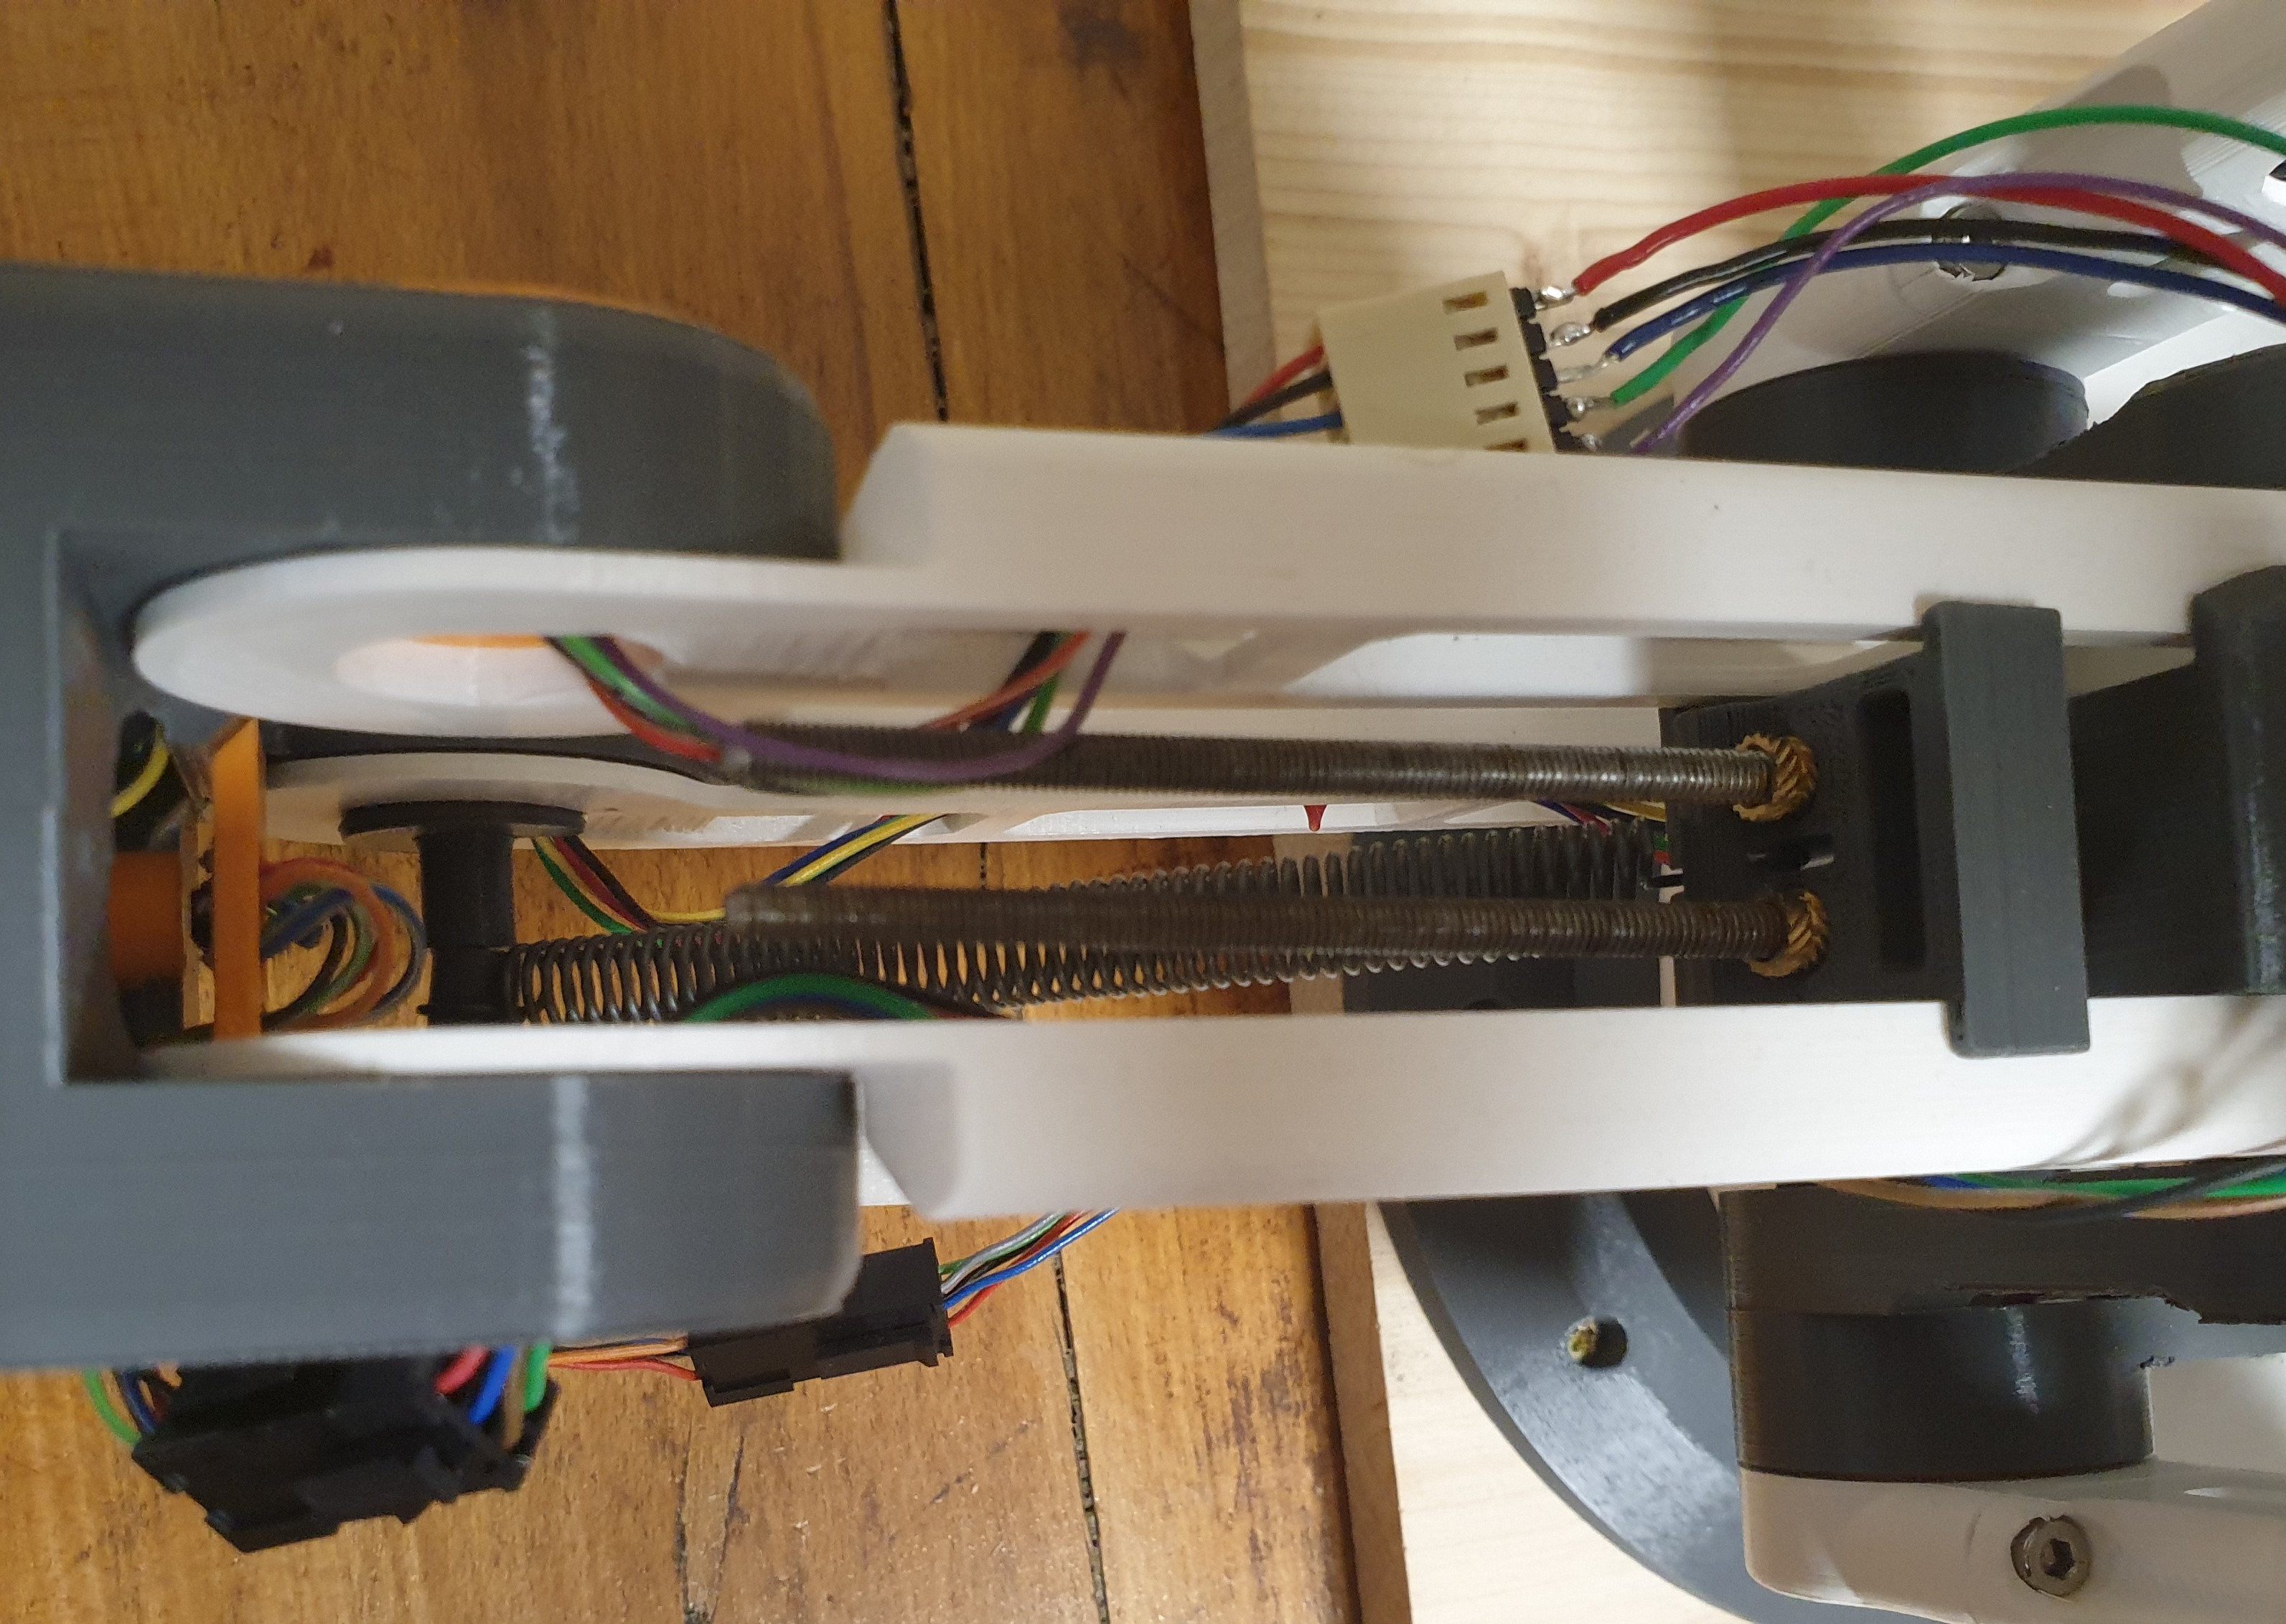
\includegraphics[width=75mm, keepaspectratio]{figures/Szumma/Orso_1}
\caption{Rugós mechanika megvalósítása}
\label{fig:rugo_1}
\end{figure}

\begin{figure}[!ht]
\centering
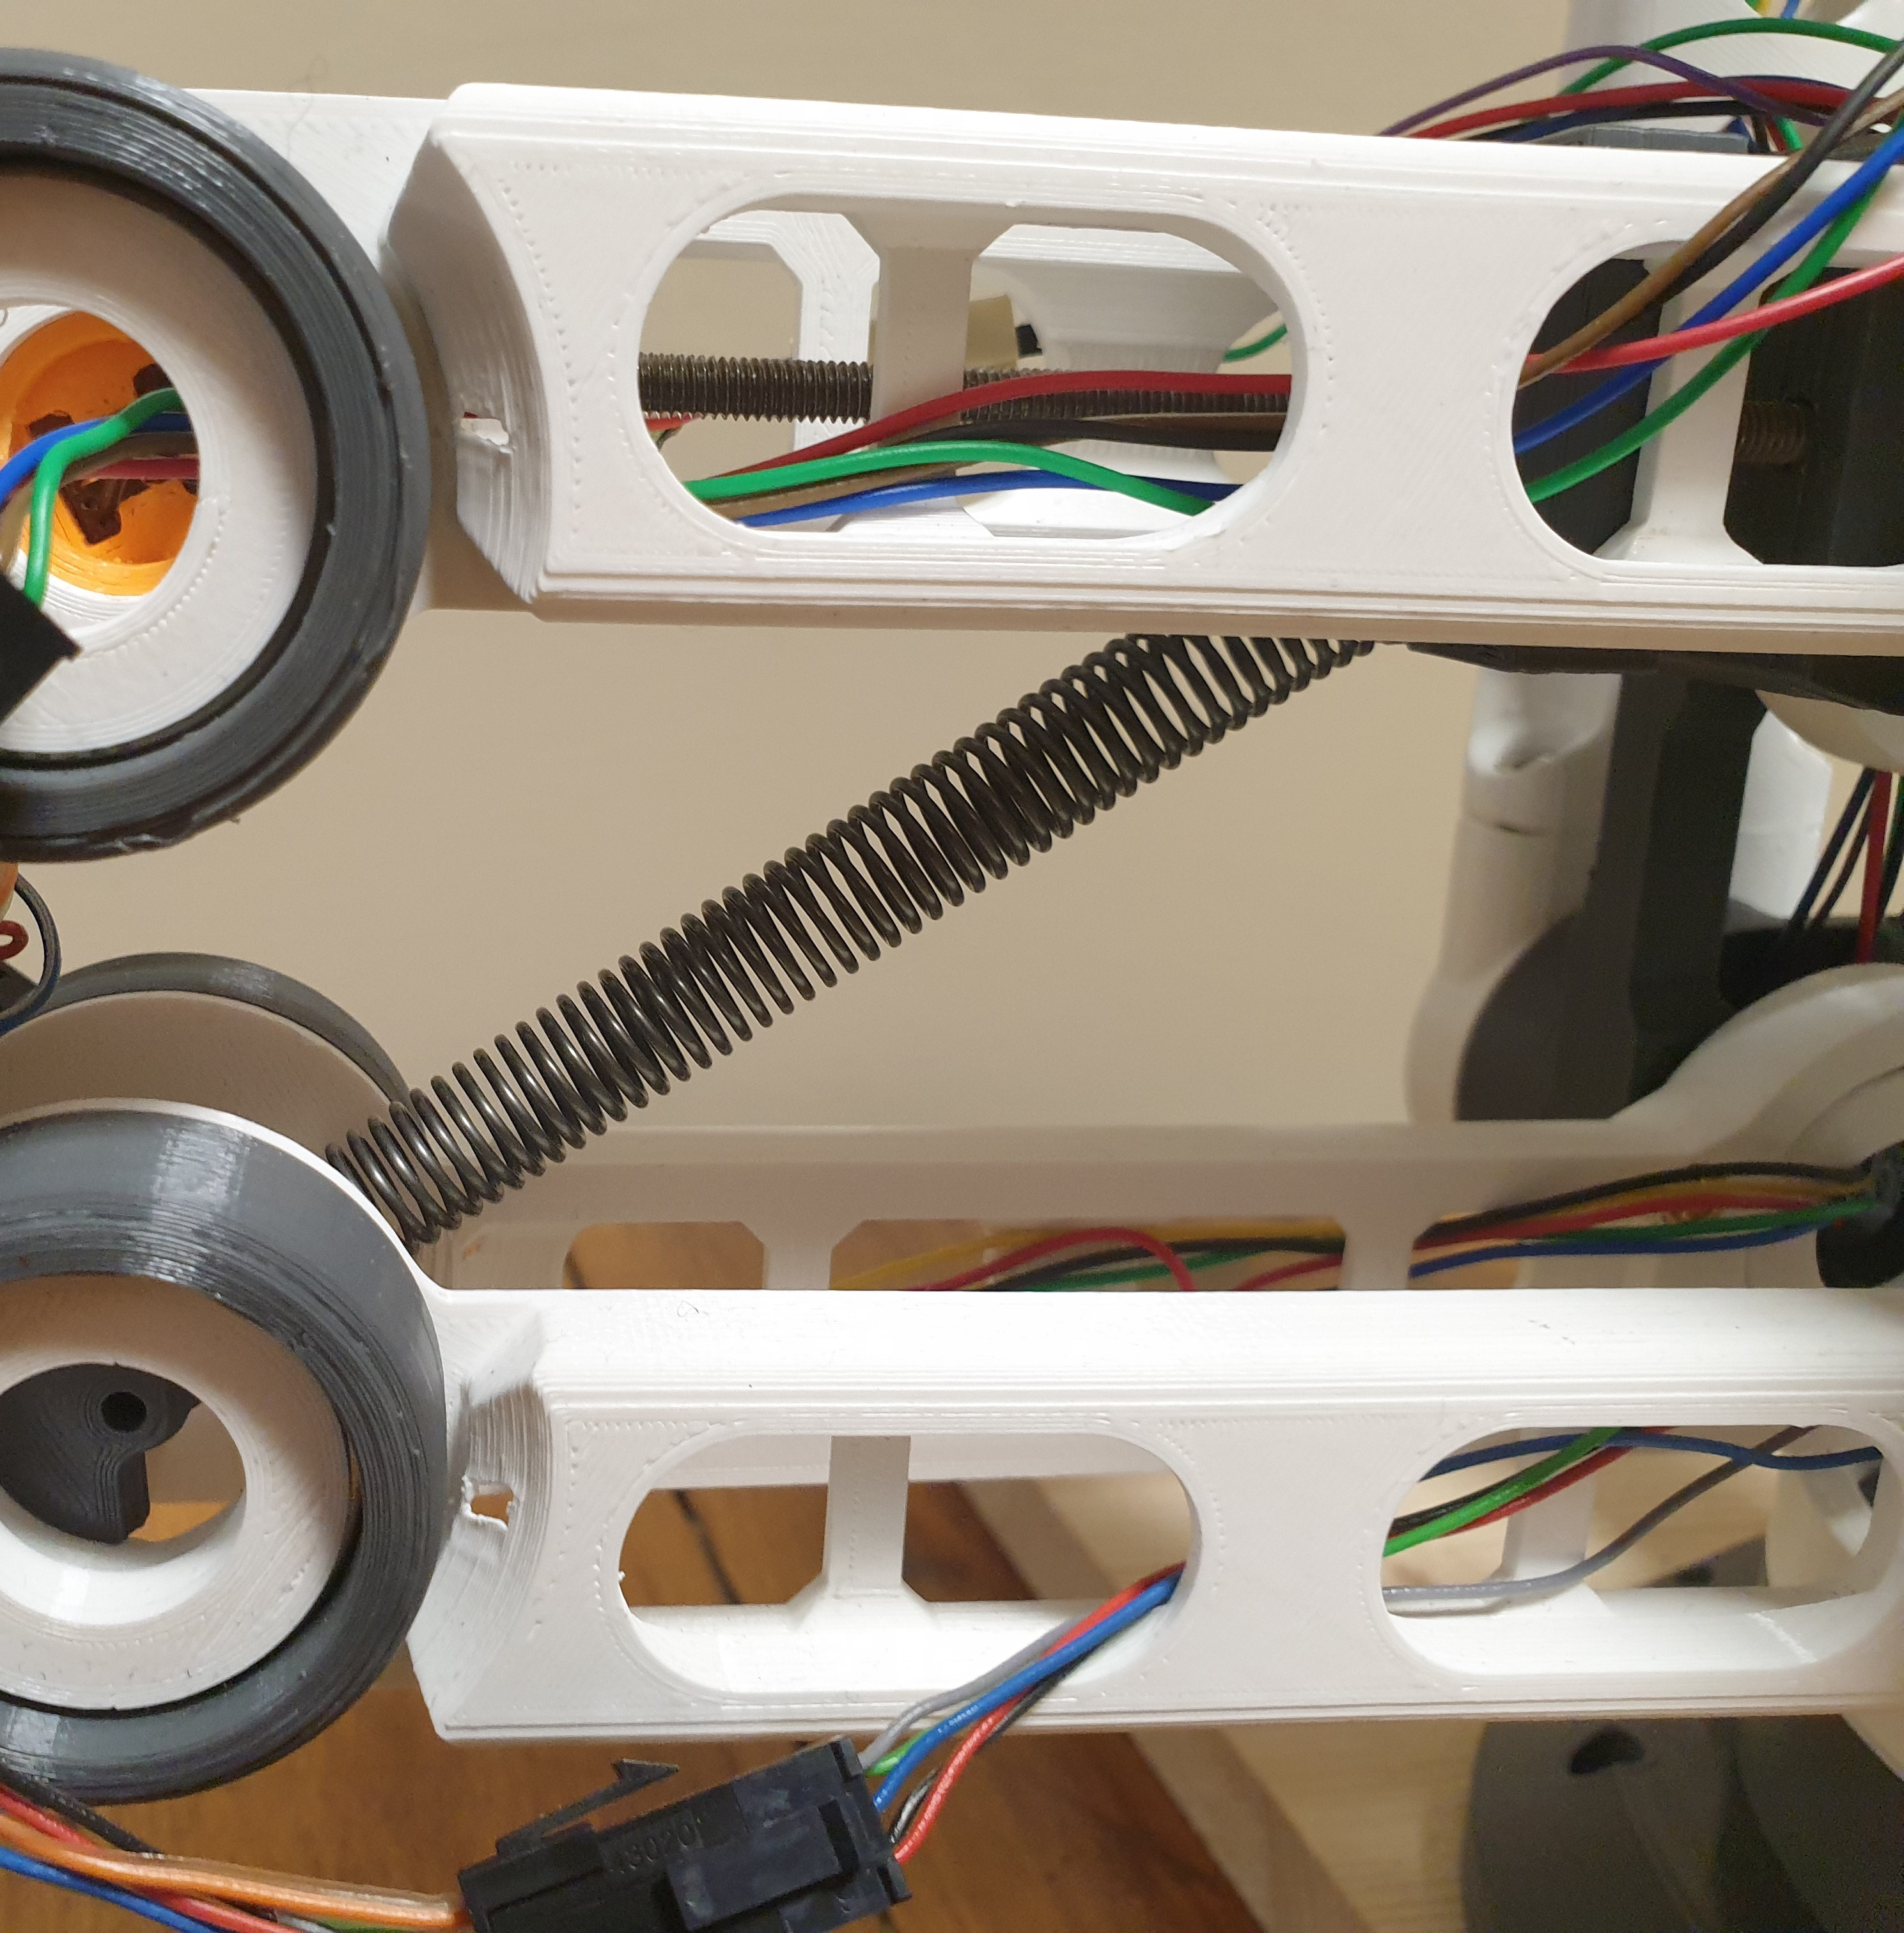
\includegraphics[width=75mm, keepaspectratio]{figures/Szumma/Orso_2}
\caption{Rugós mechanika megvalósítása}
\label{fig:rugo_2}
\end{figure}
